\section{psstream Class Reference}
\label{classpsstream}\index{psstream@{psstream}}
Collaboration diagram for psstream:\begin{figure}[H]
\begin{center}
\leavevmode
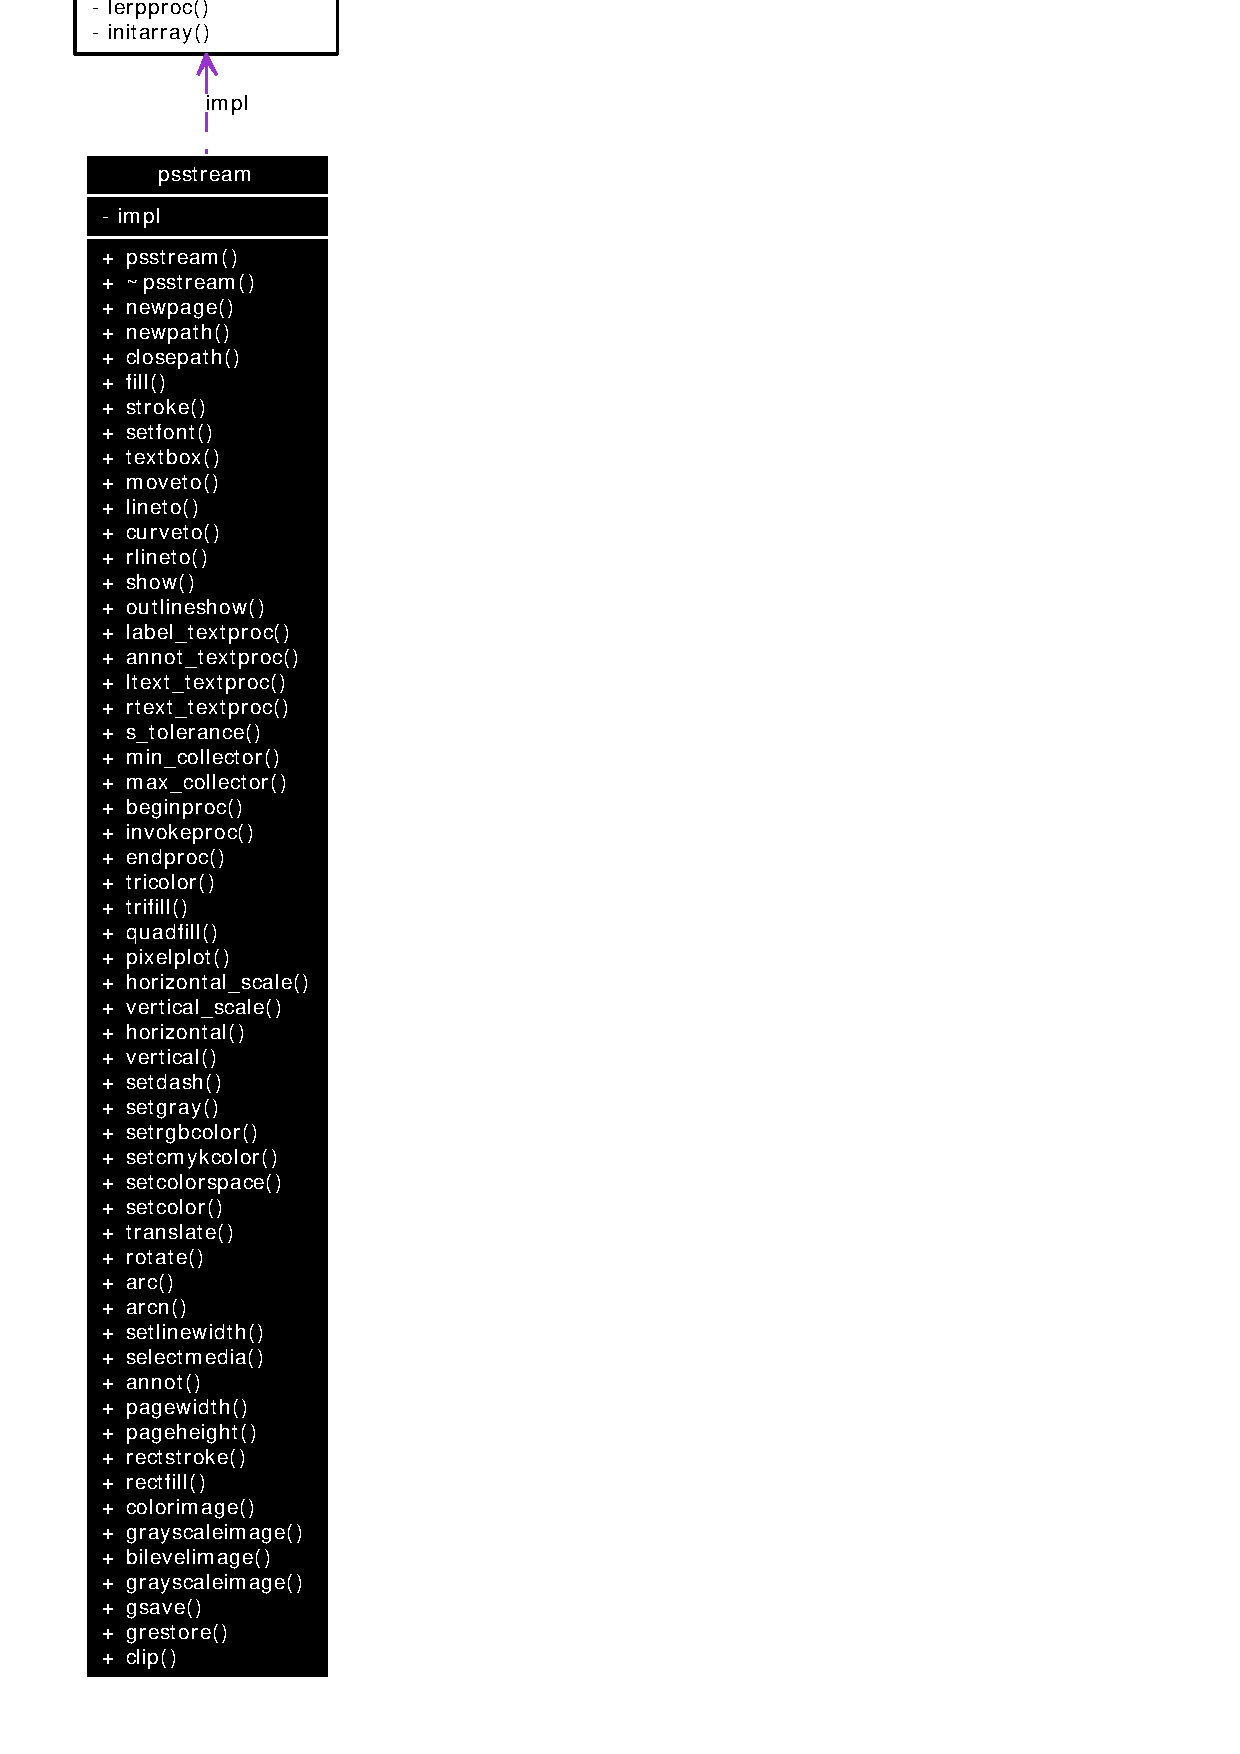
\includegraphics[width=81pt]{classpsstream__coll__graph}
\end{center}
\end{figure}
\subsection*{Public Types}
\begin{CompactItemize}
\item 
enum {\bf Orientation} \{ {\bf PORTRAIT}, 
{\bf LANDSCAPE}
 \}
\item 
enum {\bf Format} \{ {\bf FORMAT\_\-A4}, 
{\bf FORMAT\_\-A3}, 
{\bf FORMAT\_\-A0}, 
{\bf FORMAT\_\-NUM}
 \}
\item 
enum {\bf Pattern} \{ \par
{\bf BDIAGONAL}, 
{\bf CROSSHATCH}, 
{\bf DIAGHATCH}, 
{\bf HORIZONTAL}, 
\par
{\bf FDIAGONAL}, 
{\bf VERTICAL}, 
{\bf SANDSTONE}, 
{\bf SHALE}, 
\par
{\bf LIMESTONE}, 
{\bf DOLOMITE}, 
{\bf SILICATE}, 
{\bf SALT}, 
\par
{\bf ANHYDRITE}, 
{\bf SILTSTONE}, 
{\bf BITUMEN}, 
{\bf OILZONE}, 
\par
{\bf WATZONE}, 
{\bf GASZONE}, 
{\bf GYPSUM}, 
{\bf DEEPBASE}, 
\par
{\bf GASOILZONE}, 
{\bf OILWATZONE}, 
{\bf GASWATZONE}, 
{\bf GASOILWATZONE}, 
\par
{\bf WATGASZONE}, 
{\bf WATOILZONE}, 
{\bf OILGASZONE}, 
{\bf SAND}, 
\par
{\bf COAL}, 
{\bf EVALUATION}, 
{\bf NUM\_\-PATTERNS}
 \}
\item 
enum {\bf Annot} \{ {\bf ANNOT\_\-LEFT}, 
{\bf ANNOT\_\-CENTER}, 
{\bf ANNOT\_\-RIGHT}
 \}
\item 
enum {\bf Justify} \{ \par
{\bf LABEL\_\-E}, 
{\bf LABEL\_\-N}, 
{\bf LABEL\_\-W}, 
{\bf LABEL\_\-S}, 
\par
{\bf LABEL\_\-NE}, 
{\bf LABEL\_\-NW}, 
{\bf LABEL\_\-SE}, 
{\bf LABEL\_\-SW}, 
\par
{\bf LABEL\_\-NONE}
 \}
\end{CompactItemize}
\subsection*{Public Member Functions}
\begin{CompactItemize}
\item 
{\bf psstream} (const char $\ast$file)\label{classpsstream_a0}

\item 
{\bf $\sim$psstream} ()\label{classpsstream_a1}

\item 
void {\bf newpage} ()\label{classpsstream_a2}

\item 
void {\bf newpath} ()\label{classpsstream_a3}

\item 
void {\bf closepath} ()\label{classpsstream_a4}

\item 
void {\bf fill} ()\label{classpsstream_a5}

\item 
void {\bf stroke} ()\label{classpsstream_a6}

\item 
bool {\bf setfont} (const char $\ast$name, double size)\label{classpsstream_a7}

\item 
void {\bf textbox} (const char $\ast$text, double $\ast${\bf bbox})\label{classpsstream_a8}

\item 
void {\bf moveto} (double x, double y)\label{classpsstream_a9}

\item 
void {\bf lineto} (double x, double y)\label{classpsstream_a10}

\item 
void {\bf curveto} (double x1, double y1, double x2, double y2, double x3, double y3)\label{classpsstream_a11}

\item 
void {\bf rlineto} (double x, double y)\label{classpsstream_a12}

\item 
void {\bf show} (const char $\ast$text)\label{classpsstream_a13}

\item 
void {\bf outlineshow} (const char $\ast$text)\label{classpsstream_a14}

\item 
void {\bf label\_\-textproc} (double x, double y, double r, double d, const char $\ast$s, bool f)\label{classpsstream_a15}

\item 
void {\bf annot\_\-textproc} (double x, double y, double a, const char $\ast$s, bool f)\label{classpsstream_a16}

\item 
void {\bf ltext\_\-textproc} (double x, double y, double r, double a, const char $\ast$s, bool f)\label{classpsstream_a17}

\item 
void {\bf rtext\_\-textproc} (double x, double y, double r, double a, const char $\ast$s, bool f)\label{classpsstream_a18}

\item 
void {\bf s\_\-tolerance} (double s)\label{classpsstream_a19}

\item 
void {\bf min\_\-collector} (double p, double r, double g, double b)\label{classpsstream_a20}

\item 
void {\bf max\_\-collector} (double p, double r, double g, double b)\label{classpsstream_a21}

\item 
void {\bf beginproc} (const char $\ast$name)\label{classpsstream_a22}

\item 
void {\bf invokeproc} (const char $\ast$name)\label{classpsstream_a23}

\item 
void {\bf endproc} ()\label{classpsstream_a24}

\item 
void {\bf tricolor} (int n, const {\bf color\_\-type} $\ast$s)\label{classpsstream_a25}

\item 
void {\bf trifill} (double x1, double y1, double g1, double o1, double w1, double x2, double y2, double g2, double o2, double w2, double x3, double y3, double g3, double o3, double w3)\label{classpsstream_a26}

\item 
void {\bf quadfill} (double x1, double y1, double g1, double o1, double w1, double x2, double y2, double g2, double o2, double w2, double x3, double y3, double g3, double o3, double w3, double x4, double y4, double g4, double o4, double w4)\label{classpsstream_a27}

\item 
void {\bf pixelplot} (int cx, int cy, const float $\ast$xx, const float $\ast$yy, const float $\ast$gg, const float $\ast$oo, const float $\ast$ww)\label{classpsstream_a28}

\item 
void {\bf horizontal\_\-scale} (int start, int step, int final, double orig, double range, double dx, double x0, double y0, double sy)\label{classpsstream_a29}

\item 
void {\bf vertical\_\-scale} (int start, int step, int final, double orig, double range, double dy, double x0, double y0, double sx)\label{classpsstream_a30}

\item 
void {\bf horizontal} (const {\bf Scale} \&scale)\label{classpsstream_a31}

\item 
void {\bf vertical} (const {\bf Scale} \&scale)\label{classpsstream_a32}

\item 
void {\bf setdash} (int n, int $\ast$pp, int o)\label{classpsstream_a33}

\item 
void {\bf setgray} (double g)\label{classpsstream_a34}

\item 
void {\bf setrgbcolor} (double r, double g, double b)\label{classpsstream_a35}

\item 
void {\bf setcmykcolor} (double c, double m, double y, double k)\label{classpsstream_a36}

\item 
void {\bf setcolorspace} (double line\_\-width, double scale\_\-factor)\label{classpsstream_a37}

\item 
void {\bf setcolor} (double r, double g, double b, {\bf Pattern} h)\label{classpsstream_a38}

\item 
void {\bf translate} (double x, double y)\label{classpsstream_a39}

\item 
void {\bf rotate} (double a)\label{classpsstream_a40}

\item 
void {\bf arc} (double x, double y, double r, double a1, double a2)\label{classpsstream_a41}

\item 
void {\bf arcn} (double x, double y, double r, double a1, double a2)\label{classpsstream_a42}

\item 
void {\bf setlinewidth} (double w)\label{classpsstream_a43}

\item 
void {\bf selectmedia} ({\bf Format} f, {\bf Orientation} o)\label{classpsstream_a44}

\item 
void {\bf annot} (double x, double y, double r, double angle,$\backslash${\bf Annot} anchor, bool show, const char $\ast$text, double {\bf bbox}[8])\label{classpsstream_a45}

\item 
double {\bf pagewidth} () const \label{classpsstream_a46}

\item 
double {\bf pageheight} () const \label{classpsstream_a47}

\item 
void {\bf rectstroke} (double x, double y, double w, double h)\label{classpsstream_a48}

\item 
void {\bf rectfill} (double x, double y, double w, double h)\label{classpsstream_a49}

\item 
void {\bf colorimage} (double x0, double y0, double sx, double sy,$\backslash$int num\_\-levels, const float $\ast$level, const {\bf color\_\-type} $\ast$color,$\backslash$int cx, int cy, const float $\ast$func)\label{classpsstream_a50}

\item 
void {\bf grayscaleimage} (double x0, double y0, double sx, double sy,$\backslash$int num\_\-levels, const float $\ast$level, const double $\ast$color,$\backslash$int cx, int cy, const float $\ast$func)\label{classpsstream_a51}

\item 
void {\bf bilevelimage} (double x0, double y0, double sx, double sy,$\backslash$int cx, int cy, const vertex\_\-type \&ver, const edge\_\-type \&pgn)\label{classpsstream_a52}

\item 
void {\bf grayscaleimage} (double x0, double y0, double sx, double sy,$\backslash$int cx, int cy, const vertex\_\-type \&ver, const edge\_\-type \&pgn)\label{classpsstream_a53}

\item 
void {\bf gsave} ()\label{classpsstream_a54}

\item 
void {\bf grestore} ()\label{classpsstream_a55}

\item 
void {\bf clip} ()\label{classpsstream_a56}

\end{CompactItemize}
\subsection*{Classes}
\begin{CompactItemize}
\item 
struct {\bf Scale}
\end{CompactItemize}


\subsection{Detailed Description}




Definition at line 92 of file ps\_\-data.h.

The documentation for this class was generated from the following files:\begin{CompactItemize}
\item 
ps\_\-data.h\item 
ps\_\-image.cpp\item 
ps\_\-proc.0.cpp\item 
ps\_\-proc.cpp\item 
ps\_\-stream.cpp\end{CompactItemize}
